% The report. A Japanese translation with the same content is report_ja.tex.
% Build: see REPRODUCE.md, section "Building the PDF".
\documentclass[10pt,twocolumn,a4paper]{article}
\usepackage[T1]{fontenc}
\usepackage[utf8]{inputenc}
\usepackage{newtxtext,newtxmath}
\usepackage[a4paper,margin=17mm,top=18mm,bottom=20mm,columnsep=6mm]{geometry}
\usepackage{graphicx,booktabs,tabularx,array,xcolor,microtype,enumitem,multirow}
\usepackage[font=footnotesize,labelfont=bf,skip=3pt]{caption}
\usepackage{stfloats}
\usepackage[hidelinks]{hyperref}
\graphicspath{{../results/game_type_v1/}}
\setlength{\parskip}{1.5pt}
\raggedbottom
\setlist{itemsep=1pt,topsep=2pt,leftmargin=1.2em}
\newcolumntype{L}{>{\raggedright\arraybackslash}X}
\newcolumntype{P}[1]{>{\raggedright\arraybackslash}p{#1}}
\renewcommand{\arraystretch}{1.12}
\newcommand{\para}[1]{\par\smallskip\noindent\textbf{#1}\enspace}
\renewcommand{\topfraction}{0.9}\renewcommand{\bottomfraction}{0.6}\renewcommand{\textfraction}{0.07}\renewcommand{\floatpagefraction}{0.8}
\renewcommand{\dbltopfraction}{0.9}\renewcommand{\dblfloatpagefraction}{0.8}
\setlength{\textfloatsep}{8pt}\setlength{\floatsep}{6pt}\setlength{\dbltextfloatsep}{8pt}

\title{\Large\bfseries Which Game Bugs Get Tested?\\[2pt]
\large Bug Symptoms, Game Types, and Test Changes in 10,000 Open-Source Game Bug Fixes}
\author{Gen Kawamata\\[2pt]
\small AdSE Report Assignment, Option B: Bug Characteristics and Testing Strategies}
\date{}

\begin{document}
\maketitle

%======================================================================
\section{Introduction}

Studies of industrial and open-source game development report little automated testing~[1--4].
They survey developers or check whether a project contains tests at all; they do not show which kinds of bugs are fixed together with tests.
The OSSGameBench dataset~[5] links issues, pull requests and commits, but its paper counts issues by label and does not analyze which code changes fixed which bug reports.
This report asks: \textbf{how does the presence of test changes in bug fixes differ by bug symptom and by game type, and what testing strategies follow?}

\begin{itemize}
\item \textbf{RQ1.} What symptoms do reported game bugs have, and does the share of fixes that change tests differ by symptom?
\item \textbf{RQ2.} Does that share differ between discrete (turn- or move-based) and continuous (real-time) games?
\item \textbf{RQ3.} When a fix changes tests, what do the tests look like, and how do they decide whether behavior is correct?
\end{itemize}

\para{Contributions.}
(1)~A fix-level measurement (bug issue $\rightarrow$ merged pull request $\rightarrow$ final diff $\rightarrow$ test files) for 10,082 game bug fixes, beyond the label counts of~[5] and the project-level view of~[2,4].
(2)~Evidence on how test changes depend on symptom and game type, including a within-project comparison, set against practitioners' reasons~[1].
(3)~Five testing strategies, each with a scenario from a real issue and an explicit oracle.
(4)~Two pitfalls in the dataset's commit data: merges inside pull requests and reversed patches.
Section~\ref{sec:results} reports \emph{observations}, Section~\ref{sec:discussion} \emph{explanations}, and Section~\ref{sec:strategies} unevaluated \emph{proposals}.

%======================================================================
\section{Related Work}

Murphy-Hill et al.~[1] interviewed 14 developers and surveyed 364 Microsoft engineers; the interviewees reported much less test automation in games and gave reasons: the UI is hard to separate from the game, the state space is large, correct behavior is hard to state and is decided by designers, games are non-deterministic, tests become obsolete when the design changes, and human testers are cheap.
Pascarella et al.~[2] compared 30 open-source games with 30 other projects, remarked that the games contained no test cases, and found that game developers report more difficulty with automated unit tests; a literature review by Politowski et al.~[3] reports almost exclusive reliance on manual play-testing; Canella et al.~[4] found automated tests in 36 of 491 open-source games.
These studies work with surveys or whole projects.
Truelove et al.~[6] classified bug fixes in update notes of popular Steam games, and~[5] reports label frequencies, but neither relates bug types to the tests that accompany fixes.
Automatic game oracles are studied for graphical glitches~[7] and regression test selection~[8]; the proposals here judge game state instead of pixels.

%======================================================================
\section{Data and Measures}\label{sec:data}

\subsection{Dataset and bug fixes}\label{sec:selection}
I use \texttt{OSSGameBench.zip} from Zenodo record 17553539 (65,816,061,871 bytes; MD5 \texttt{40fd064b56ec327b6284039b18b19ea1}); the newest record (18359123) contains no data files.
Following the authors' notebook, 20 duplicated repositories are removed, leaving 950 projects; the 319,709 issues and 2,758,344 commits match the paper~[5].
The unit of analysis is a \textbf{fix}: a bug issue with all merged pull requests linked to it (Table~\ref{tab:sel}).
Using only \emph{merged} pull requests partly addresses the fact that a closed issue is not necessarily fixed.
Reported bugs are not the bugs that occurred: unreported and unlabeled bugs are outside this study.
How each classification was checked is summarized in Table~\ref{tab:val}.

\begin{table}[htbp]
\centering
\caption{Selection of the analyzed bug fixes.}\label{tab:sel}
\footnotesize
\begin{tabularx}{\columnwidth}{@{}cLrr@{}}
\toprule
Step & Criterion & Issues & Projects\\
\midrule
1 & All issues & 319,709 & 950\\
2 & A bug label (123 normalized labels such as \texttt{bug}, \texttt{crash}) and no no-fix label (93 such as \texttt{duplicate}, \texttt{wontfix}) & 81,620 & 701\\
3 & Linked to a merged pull request whose commits are in the dataset and list changed files & 13,883 & 348\\
4 & Project is a game (not an engine, library or tool), judged by an LLM from its README & 10,511 & 181\\
5 & Every linked merged pull request has an identifiable final diff (Section~\ref{sec:pitfalls}) & \textbf{10,082} & \textbf{177}\\
\bottomrule
\end{tabularx}
\end{table}

\begin{table*}[tb]
\centering
\caption{Validation of the classifications.}\label{tab:val}
\small
\begin{tabularx}{\textwidth}{@{}P{24mm}P{40mm}L@{}}
\toprule
Step & Checked against & Result\\
\midrule
Bug labels & LLM (OpenAI Codex), 100 fixes; author, 19 issues & 97 real bugs, 1 feature request, 2 unclear; author: 19/19 real bugs; recall not measured\\
Game scope & LLM only & 181 games, 125 engines/tools, 20 mixed, 22 unknown among 348 projects; not checked by the author\\
Landing diff & GitHub, 74 pull requests & file sets identical for 70; test flag agrees for 73\\
Patch direction & GitHub, 83 patches & all 70 decidable patches reversed\\
Test-path rule & LLM, 50 flagged and 50 unflagged fixes; keyword search of all 9,456 unflagged fixes & 46/50 flagged are test-related (34 test code, 12 fixtures or mocks only); 0/50 missed; 45 misses found (rate 6.21\%\,$\rightarrow$\,6.66\%)\\
Symptom rules & LLM, 100 held-out issues & accuracy 0.71, $\kappa=0.59$ (development sample: 0.80, 0.73)\\
Symptom rules & author (consulting ChatGPT), 19 audit issues & 15/19, $\kappa=0.64$; author vs.\ Claude labels 18/19 ($\kappa=0.91$); not independent of an LLM\\
Game type & LLM only & not checked by the author\\
RQ3 content & LLM only & 30 pull requests labeled from inverted patches; not checked by the author\\
\bottomrule
\end{tabularx}
\end{table*}

\subsection{Two pitfalls in the commit data}\label{sec:pitfalls}
\para{Merges inside pull requests.}
The dataset lists all commits of a pull request, including ``Merge branch `master' into \ldots'' commits whose files belong to other work.
I therefore use only the \textbf{landing commit}: the single commit whose first line is ``Merge pull request \#N \ldots'' or ends with ``(\#N)''.
Of 12,607 merged pull requests, 12,128 have one landing diff; 153 with conflicting candidates and 326 with none are excluded (step~5; 371 of 9,434 in games).
With the union of all commits the test-change rate for games would be 6.97\% instead of 6.21\%.

\para{Reversed patches.}
The per-file patches are stored child to parent: lines marked ``$-$'' are additions.
File lists, and therefore the main measure, are not affected; for RQ3 I inverted the patches before reading them.

\subsection{Outcome measure}\label{sec:outcome}
A fix is \textbf{test-changing} if its final diff contains a path matching a fixed rule for test files (directories such as \texttt{test}, \texttt{spec}, \texttt{\_\_tests\_\_}; names such as \texttt{test\_*}, \texttt{*\_test.*}, \texttt{*Test.java}).
This measures the \emph{co-change of test-related files}, not that a regression test was written or run, or that the fix is correct (Table~\ref{tab:constructs}).
Adding the 45 missed paths found in validation does not change the direction of any comparison below.

\begin{table}[htbp]
\centering
\caption{Measures used and the concepts they do not directly measure.}\label{tab:constructs}
\footnotesize
\begin{tabularx}{\columnwidth}{@{}P{30mm}L@{}}
\toprule
Measure & What it does \emph{not} directly measure\\
\midrule
Issue with a bug label & Occurrence of bugs\\
Linked merged pull request & Successful fix; it may be partial or wrong\\
Test-related path in the final diff & A regression test for the reported bug; whether tests were run or pass\\
Symptom from keyword rules & The true failure type\\
Game type and scope (LLM, README) & How the game is actually built and played\\
No test-related path & That the bug was untestable, untested, or tested elsewhere or by hand\\
\bottomrule
\end{tabularx}
\end{table}

\subsection{Bug symptoms}\label{sec:symptoms}
Each issue gets one symptom from keyword rules applied to the title and, if nothing matches, to the body: crash/hang, save/load, performance, network, audio, visual, UI, tooling.
An issue that matches no rule is labeled \textbf{gameplay/rules}, so this class also collects misclassified issues (examined in Section~\ref{sec:rq1}).
Save/load, performance, network and tooling are merged into ``other'' for inference.
The rules were written on a \emph{development sample} of 100 issues, frozen, and evaluated once on a disjoint \emph{audit sample} of 100 issues (Table~\ref{tab:agree}).
The reference labels come from OpenAI Codex and Claude; the Claude labels were sealed by a committed SHA-256 hash until the author had labeled.

\begin{table}[htbp]
\centering
\caption{Agreement of the symptom rules with reference labels.}\label{tab:agree}
\footnotesize
\begin{tabularx}{\columnwidth}{@{}Lrrr@{}}
\toprule
Reference labels & $n$ & Accuracy & $\kappa$\\
\midrule
Development sample, OpenAI Codex & 100 & 0.80 & 0.73\\
Audit sample, Claude (held out) & 100 & 0.71 & 0.59\\
Author, consulting ChatGPT (audit subset) & 19 & 0.79 & 0.64\\
\bottomrule
\end{tabularx}
\end{table}

Agreement on the held-out sample is moderate; crash, UI, gameplay and audio have precision and recall of at least 0.73, and visual bugs have high precision but low recall.
The author labeled the first 19 issues of a random 50-issue subset of the audit sample from titles and bodies, consulting ChatGPT and without seeing the Claude labels or the rule predictions.
The rules agree with these labels on 15 of 19, and the author's labels agree with the Claude labels on 18 of 19 ($\kappa=0.91$).
Because the author consulted an LLM, this does not show agreement with independent human judgment; the symptom analysis rests on LLM reference labels.

\subsection{Game type}\label{sec:gametype}
An LLM labeled each project from its topics and README as \textbf{discrete}---play advances by turns, moves or choices: board, card, turn-based strategy, roguelike, puzzle (73 projects, 5,390 fixes)---or \textbf{continuous}---play advances in real time: action, platformer, racing, real-time strategy (102 projects, 4,474 fixes); two mixed projects are excluded from RQ2.
I also record whether a game runs in a browser or a chat service (\textbf{web}, 49 projects), because web development has its own testing culture.

%======================================================================
\section{Analysis Methods}\label{sec:methods}

\begin{itemize}
\item \textbf{Shares} with 95\% intervals from a project-cluster bootstrap (2,000 replicates), because a few projects contribute many fixes.
\item \textbf{GEE logistic regression} with projects as clusters, reported with both exchangeable and independence working correlation (the latter weights every fix equally). Controls: log of non-test files changed and report year; RQ2 adds log project size and web. Because 175 projects give little power for a project-level variable, RQ2 is reported over a grid of specifications and at project level.
\item \textbf{Within-project comparison} (RQ1): logistic regression with project fixed effects, with project-clustered Wald and project-bootstrap intervals; McFadden's $R^2$; a sign test over projects.
\item \textbf{Sensitivity analyses}: without the largest projects, only single-issue pull requests, only projects with tests in their history, without diffs over 100 files.
\item \textbf{Content analysis} (RQ3): 30 test-changing pull requests in random order, at most three per project (18 projects). This is a diversity sample, not a prevalence estimate. An LLM (Claude) labeled the relation of the test to the bug, the input and the oracle; the tests were not executed.
\end{itemize}

%======================================================================
\section{Results}\label{sec:results}

\subsection{Symptoms and overall test changes (RQ1)}

\begin{table}[htbp]
\centering
\caption{Symptoms of bug issues in the 181 game projects.}\label{tab:dist}
\footnotesize
\begin{tabular}{@{}lrrr@{}}
\toprule
Symptom & All bug issues & Analyzed fixes & Traceable\\
 & ($n=49{,}381$) & ($n=10{,}082$) & to a fix\\
\midrule
Gameplay / rules & 45.9\% & 45.8\% & 20.4\%\\
UI & 22.8\% & 24.7\% & 22.2\%\\
Crash / hang & 10.7\% & 9.9\% & 18.8\%\\
Visual & 8.6\% & 7.8\% & 18.5\%\\
Tooling & 5.3\% & 5.2\% & 20.2\%\\
Audio & 2.4\% & 2.6\% & 21.8\%\\
Network & 2.2\% & 2.1\% & 20.0\%\\
Performance & 1.4\% & 0.9\% & 13.5\%\\
Save / load & 0.8\% & 0.9\% & 25.4\%\\
\bottomrule
\end{tabular}
\end{table}

About half of the reported game bugs concern game rules and state, and about a quarter the UI (Table~\ref{tab:dist}).
Only 20.4\% of the 49,381 game bug issues can be traced to a fix, but their symptom mix is almost the same as that of all issues (largest gap 1.9 points).

Of the 10,082 fixes, 626 (6.2\%; 95\% CI 3.5--9.5\%) change a test file.
Only 61 of the 177 projects have any such fix, and five (18xx, mage, vcmi, space-station-14, cuttle) account for 64\% of them.
The second-largest project, fheroes2, has 1,262 fixes and none with a test change.

\subsection{Test changes by symptom (RQ1)}\label{sec:rq1}

\begin{table*}[tb]
\centering
\caption{Test-changing fixes by symptom. Shares with project-cluster bootstrap 95\% CIs. Odds ratios (OR) relative to gameplay/rules from GEE models adjusted for non-test files changed (log) and report year; ``Exch.''\ = exchangeable, ``Ind.''\ = independence working correlation.}\label{tab:sym}
\small\setlength{\tabcolsep}{4pt}
\begin{tabular}{@{}lrrrlll@{}}
\toprule
Symptom & Fixes & Projects & Test & Share (95\% CI) & Exch.\ OR (95\% CI) & Ind.\ OR (95\% CI)\\
\midrule
Gameplay / rules & 4,620 & 143 & 396 & 8.6\% (4.6--13.4) & reference & reference\\
UI & 2,493 & 121 & 111 & 4.5\% (2.4--6.7) & 0.68 (0.57--0.82) & 0.46 (0.31--0.69)\\
Crash / hang & 996 & 86 & 41 & 4.1\% (2.4--6.0) & 0.82 (0.69--0.96) & 0.43 (0.27--0.67)\\
Visual & 786 & 76 & 29 & 3.7\% (1.1--8.4) & 0.65 (0.52--0.80) & 0.35 (0.20--0.61)\\
Audio & 261 & 46 & 2 & 0.8\% (0.0--2.7) & 0.32 (0.20--0.49) & 0.07 (0.01--0.45)\\
Other & 926 & 81 & 47 & 5.1\% (2.9--7.4) & 0.71 (0.59--0.85) & 0.48 (0.32--0.71)\\
\midrule
All & 10,082 & 177 & 626 & 6.2\% (3.5--9.5) & & \\
\bottomrule
\end{tabular}
\end{table*}

The share is highest for gameplay/rule bugs and lowest for audio bugs (Table~\ref{tab:sym}).
The bootstrap intervals overlap because projects differ strongly, but both GEE models give odds ratios below 1 for every symptom relative to gameplay; the direction does not depend on the model, the size does.
Fixes that change more non-test files change tests more often (OR 1.86 per log-unit, 95\% CI 1.56--2.21).
The ordering ``gameplay highest, audio lowest'' holds in every sensitivity analysis: for example, gameplay 9.8\% and audio 1.2\% without the three largest projects, and 7.6\% and 0.0\% with single-issue pull requests only.
Both test-changing audio fixes come from vcmi, so the audio estimates rest on two events.

\para{Within-project comparison.}
Because gameplay is also the fallback class, a gameplay ``effect'' could arise if test-writing projects simply write more reports that match no keyword.
A model with project fixed effects (56 projects with both outcomes, 7,687 fixes) removes differences in the project mix.
Within projects, UI, visual, audio and other fixes still change tests less often than gameplay fixes; crash/hang is no longer clearly different (Table~\ref{tab:within}).
Gameplay has the higher share in 21 and the lower in 12 of 34 test-writing projects with enough fixes (sign test $p=0.16$), so the effect is a tendency rather than a rule.
Part of the gap goes with how reports are titled: within each symptom, issues matched only through the body change tests more often (for example UI 6.6\% vs.\ 3.4\%).
Project identity explains far more than symptom: McFadden's $R^2$ is 0.25 for projects only and 0.02 for symptoms only.

\begin{table}[htbp]
\centering
\caption{Within-project odds ratios relative to gameplay (project fixed effects, adjusted for non-test files changed and year).}\label{tab:within}
\footnotesize
\begin{tabular}{@{}lrll@{}}
\toprule
Symptom & OR & Wald 95\% CI & Bootstrap 95\% CI\\
\midrule
UI & 0.58 & 0.40--0.85 & 0.38--0.80\\
Crash / hang & 0.85 & 0.59--1.23 & 0.61--1.37\\
Visual & 0.59 & 0.38--0.93 & 0.33--0.84\\
Audio & 0.12 & 0.02--0.75 & 0.00--0.36\\
Other & 0.68 & 0.50--0.93 & 0.49--0.96\\
\bottomrule
\end{tabular}
\end{table}

\para{Answer to RQ1.}
About half of the reported game bugs concern rules and state, and a quarter the UI.
Fixes of rule bugs change tests more often than fixes of UI, visual and especially audio bugs, also within projects; crash fixes are not clearly different within projects.
\textbf{Whether a fix changes tests is mainly a property of the project; within a project, the symptom shifts it.}

\subsection{Test changes by game type (RQ2)}\label{sec:rq2}

At fix level, 8.8\% of fixes in discrete games change tests (475/5,390; 95\% CI 4.0--16.6\%) against 3.3\% in continuous games (148/4,474; 2.2--4.4\%).
The share is higher in discrete games for every symptom, and gameplay is highest and audio lowest in both types (Figure~\ref{fig:type}).

\begin{figure}[htbp]
\centering
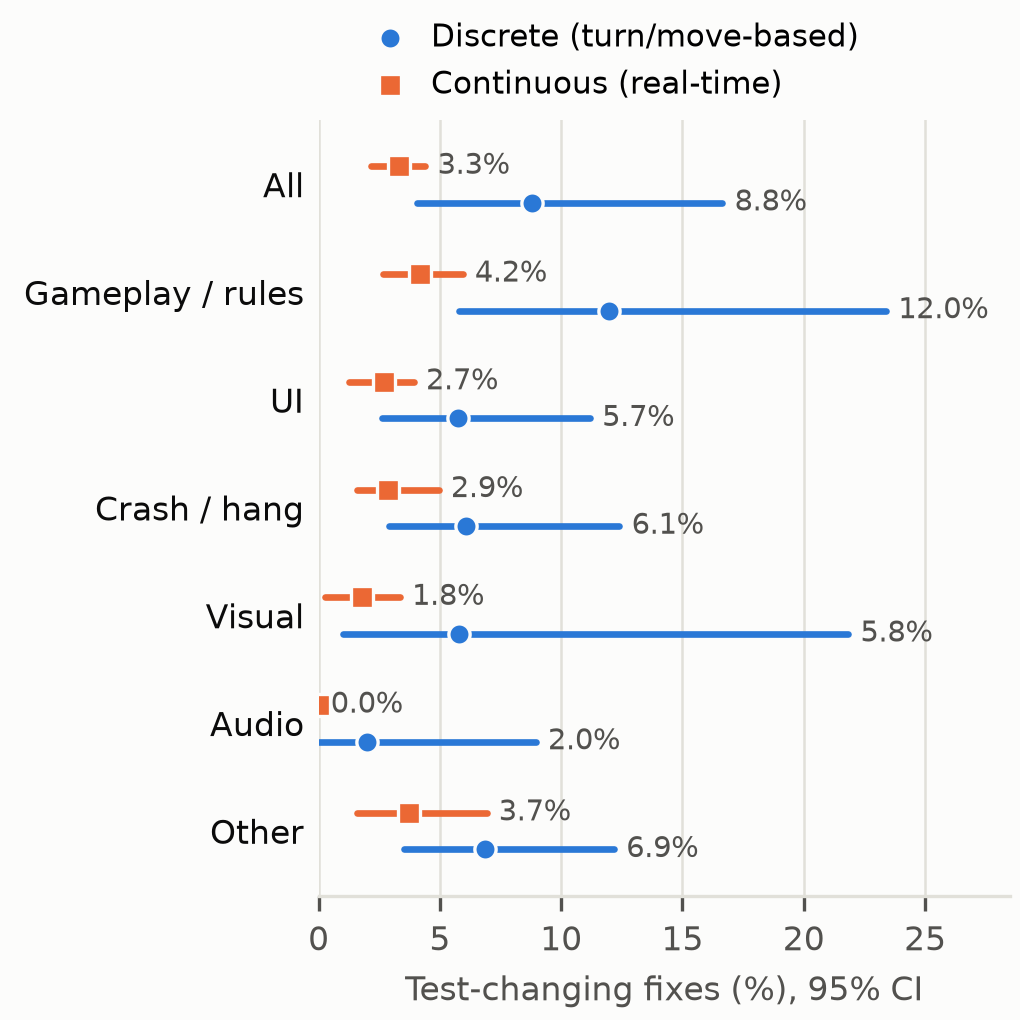
\includegraphics[width=\columnwidth]{fig_game_type_by_symptom.png}
\caption{Share of test-changing fixes by symptom and game type (unadjusted), with project-cluster bootstrap 95\% CIs.}\label{fig:type}
\end{figure}

Game type and web technology overlap strongly: 40 of the 49 web games are discrete, and only 9 continuous games (87 fixes) are web games (Table~\ref{tab:web}).
Among non-web projects the share is still higher in discrete games (7.6\% vs.\ 3.2\%), but the intervals are wide.

\begin{table}[htbp]
\centering
\caption{Test-changing fixes by game type and web technology (unadjusted; project-cluster bootstrap 95\% CIs).}\label{tab:web}
\footnotesize\setlength{\tabcolsep}{4pt}
\begin{tabular}{@{}llrrrl@{}}
\toprule
Type & Web & Projects & Fixes & Test & Share (95\% CI)\\
\midrule
Discrete & yes & 40 & 2,435 & 250 & 10.3\% (5.5--18.2)\\
Discrete & no & 33 & 2,955 & 225 & 7.6\% (1.4--24.9)\\
Continuous & yes & 9 & 87 & 7 & 8.0\% (0.0--15.1)\\
Continuous & no & 93 & 4,387 & 141 & 3.2\% (2.0--4.4)\\
\bottomrule
\end{tabular}
\end{table}

The adjusted odds ratio of discrete vs.\ continuous games is above 1 in every specification (1.8--4.3), but once web technology and the other controls are included, about half of the intervals include 1 (Table~\ref{tab:or}).
The web odds ratio ranges from 1.2 to 3.1, so the two variables cannot be separated well with 175 projects.
At project level, 35 of 73 discrete projects (48\%) have a test-changing fix against 25 of 102 continuous ones (25\%), but among projects with at least 10 fixes the interval includes 1.

\begin{table}[htbp]
\centering
\caption{Odds ratio of discrete vs.\ continuous games over selected specifications (full grid in the repository). Fix level: GEE, independence (Ind.) or exchangeable (Exch.); ``Full'' adds symptom, web, non-test files changed, year and project size. Project level: logistic regression with web and project size.}\label{tab:or}
\footnotesize
\setlength{\tabcolsep}{3pt}
\begin{tabularx}{\columnwidth}{@{}Lll@{}}
\toprule
Fix-level model & Ind.\ OR (95\% CI) & Exch.\ OR (95\% CI)\\
\midrule
Game type only & 2.83 (1.28--6.21) & 4.33 (2.27--8.26)\\
+ web & 2.39 (0.66--8.72) & 3.06 (1.42--6.62)\\
Full & 3.01 (0.94--9.59) & 2.29 (1.10--4.76)\\
Full, non-web only & 3.11 (0.89--10.9) & 1.85 (0.80--4.24)\\
Full, without 5 largest & 1.78 (0.75--4.23) & did not fit\\
\midrule
Project-level model & \multicolumn{2}{l}{OR (95\% CI)}\\
\midrule
Any test change, 175 projects & \multicolumn{2}{l}{2.94 (1.19--7.23)}\\
Any test change, $\geq$10 fixes (81) & \multicolumn{2}{l}{2.34 (0.73--7.51)}\\
\bottomrule
\end{tabularx}
\end{table}

\para{Answer to RQ2.}
Fixes in discrete games tend to change tests more often (odds ratio about 2--3 after adjustment), but the evidence is not conclusive: the difference is clear only in some specifications and cannot be separated well from web technology.

\subsection{What the tests look like (RQ3)}\label{sec:rq3}

\begin{table*}[tb]
\centering
\caption{Relation between the test change and the reported bug in 30 test-changing pull requests (LLM labels; diversity sample, not a prevalence estimate).}\label{tab:relation}
\small
\begin{tabularx}{\textwidth}{@{}Lrl@{}}
\toprule
Relation & $n$ & Examples (pull request)\\
\midrule
Tests the reported failure directly & 14 & farmhand\#431, 18xx\#2558, space-station-14\#1856, triplea\#7292\\
Tests the same feature but not the reported condition & 4 & eternajs\#414, mage\#13516\\
Only adapts existing tests to changed code (API, mocks, configuration) & 10 & vcmi\#2209, lila\#14331, gemrb\#2027\\
New test unrelated to the bug / the bug is in the tests themselves & 2 & spellmasons\#460, cuttle\#717\\
\bottomrule
\end{tabularx}
\end{table*}

\begin{table*}[tb]
\centering
\caption{The 14 direct regression tests: how the input is fixed and how correctness is decided (LLM labels from inverted patches).}\label{tab:direct}
\footnotesize\setlength{\tabcolsep}{3pt}
\begin{tabularx}{\textwidth}{@{}P{30mm}P{14mm}LL@{}}
\toprule
Pull request & Symptom & Input state and action & Oracle\\
\midrule
18xx\#2558 & crash & Recorded game linked in the issue; replay all actions & Replay completes; final player values; page shows ``Game Over -- Bankruptcy''\\
mage\#10802 & gameplay & Battlefield with the reported card, lands, other Clerics; activate, attack & Opponent's life total; number of tapped lands\\
mage\#11740 & gameplay & Creatures moved to the graveyard from four zones; cast the card & Each creature is back on the battlefield\\
space-station-14\#1856 & gameplay & Headless server; human buckled to a chair with items in hand; lethal damage & Hands are empty (items dropped)\\
space-station-14\#28197 & gameplay & Lobby players with preference on/off; run role selection & Only opted-in, eligible players selected\\
farmhand\#431 & gameplay & Field row where the target is not first in its row & Helper returns the plot, or null when absent\\
eternajs\#666 & gameplay & Multi-strand RNA sequences with a cut point & Expected structure string, energies, per-node scores\\
cuttle\#378 & UI & Spectator view with a game fixture; opponent plays one-offs & DOM: dialog visible, then overlay absent\\
lila\#17650 & UI & Chess positions (FEN); move strings in mixed case & Parser returns the expected move\\
quadradius\#124 & UI & Database with 3 users and ranked matches; request ranking & Ranking entries equal expected values\\
triplea\#7292 & crash & Point sets with duplicate coordinates (from the stack trace) & One index per point, strictly increasing\\
openra\#8000 & crash & Two YAML trees with additions and removals; merge & Merged tree contains / omits expected keys\\
microcosm\#175 & crash & Legacy saved game configurations; migrate & Fields are proper enum members\\
terasology\#5039 & tooling & Test classes with two lifecycles; run hooks & Same engine instance across hooks\\
\bottomrule
\end{tabularx}
\end{table*}

Fewer than half of the sampled test-changing fixes test the reported bug (Table~\ref{tab:relation}), so a test-file change overstates regression testing.
In the 14 direct regression tests, correctness is decided by comparing \textbf{game state or computed values}: life totals, cards on the battlefield, items held, a DOM element, a parsed move (Table~\ref{tab:direct}).
No test compares images; even a UI bug reported with a screenshot (cuttle\#378) is tested through DOM state.
Inputs are fixed in game-specific ways rather than through random seeds: a card layout, a chess position, a recorded game, an old save configuration.
In 18xx\#2558 the game linked in the report became a replay fixture; in triplea\#7292 the stack trace named the failing method, and the test feeds it duplicate coordinates.
Bug reports contain such material: by simple, unvalidated text rules, 55\% of visual and 49\% of UI reports contain an image, 31\% of crash reports a log or stack trace, and 11\% of all reports link a save or other attachment.

\para{Answer to RQ3.}
Fewer than half of the sampled test changes test the reported bug; those that do fix the input exactly, often with game-specific material, and check state or values, not images.

%======================================================================
\section{Discussion}\label{sec:discussion}

Table~\ref{tab:reasons} compares the reasons practitioners gave in~[1] with the fix data.
``Consistent'' means only that an association has the expected direction, not that the reason is the cause; the data cannot tell whether a fix without tests needed none, could not be tested, or was tested by hand.

\begin{table}[htbp]
\centering
\caption{Practitioner reasons~[1], the expected pattern, and what is observed.}\label{tab:reasons}
\footnotesize
\begin{tabularx}{\columnwidth}{@{}P{27mm}L@{}}
\toprule
Reason (expected pattern) & Observed\\
\midrule
UI is hard to separate (UI bugs tested less) & Consistent: 4.5\% vs.\ 8.6\%; within projects OR 0.58\\
Correct behavior is hard to state (visual, audio tested least) & Consistent: 3.7\%, 0.8\%; within projects OR 0.59, 0.12\\
Non-determinism (real-time games tested less) & Consistent in direction (3.3\% vs.\ 8.8\%); not conclusive\\
Tests become obsolete (many changes only adapt tests) & Weak: 10 of 30 only adapt tests to changed code\\
Human testers are cheap & Not measurable here\\
\bottomrule
\end{tabularx}
\end{table}

\para{Competing explanations.}
\emph{Web technology}: turn-based games are often web applications, which come with test frameworks; but they may be built for the web \emph{because} they are turn-based, in which case adjusting for web removes part of a real game-type effect.
\emph{Project practice}: whether a project has a testing practice at all, not measured here, may explain the dominance of the project; the concentration in five projects and large projects without any test change (fheroes2) fit this reading.
\emph{Report wording}: part of the symptom gap may reflect how developers in test-writing projects write reports, which the within-project comparison does not remove.

\para{Implication.}
Tests are missing mostly where it is hard to state what is correct (audio, visual, UI) and hard to reproduce a situation (real-time games); where tests exist, they fix the input exactly and compare state.
Testing strategies for games should therefore provide a \textbf{reproducible input} and a \textbf{state-based oracle}.
This is an interpretation of associations, not a causal finding.

%======================================================================
\section{Proposed Testing Strategies}\label{sec:strategies}

\textbf{None of the strategies has been implemented or evaluated, so I make no claim about their effectiveness.}
S1--S3 address situations that should be testable but mostly are not (91\% of fixes in discrete games change no tests); S4--S5 address the situations where tests are rarest.
Each scenario comes from a real issue in the dataset; Table~\ref{tab:detect} summarizes them.

\para{S1: Replay of recorded games (discrete games; rule bugs).}
Rule bugs are the largest class (46\%), turn-based games can record all actions, and 18xx already turns reported games into replay tests (\#2558).
\emph{Scenario} (18xx \#7236, ``discarding of Pullmans is not enforced''): replay the game linked in the report up to action 406 and query the actions available at action 407.
\emph{Oracle}: the only train that may be discarded is the Pullman; the whole record replays without an exception; invariants hold (shares per company and total money are constant).
\emph{Limitations}: when rules are corrected, old records may legitimately end differently; records contain player names; the game must be deterministic.

\para{S2: State--action--expectation scenarios (rule, UI, crash bugs).}
Most of the 14 direct regression tests have this form, and 31\% of crash reports carry a stack trace that names the failing function.
\emph{Scenario} (fheroes2 \#2249, ``Berserker spell doesn't work as it should''; a project with no test-changing fix): set up the battle in the report, cast Berserker on the Cyclops, skip the next unit.
\emph{Oracle}: on the Cyclops' turn the battle log shows an attack on an adjacent troop of either side, and its hit points decrease.
\emph{Limitations}: battle logic must run without rendering; translating vague reports is manual; ``does not crash'' alone is a weak oracle.

\para{S3: Compatibility tests with old save files (save/load bugs).}
About 11\% of reports link attachments such as saves, one sampled fix tests an old configuration format (microcosm\#175), and issues such as fheroes2 \#3775 report broken old saves.
\emph{Scenario}: collect saves attached to issues; with each new version load them headless, save and reload.
\emph{Oracle}: no exception except for declared unsupported versions; invariants hold (heroes on passable tiles, no negative resources); the round trip preserves the state.
\emph{Limitations}: attachment links expire, redistribution needs permission, and loading correctly does not guarantee correct play.

\para{S4: Fixed-step headless tests (continuous games).}
space-station-14 starts a server without a window, advances a fixed number of ticks and checks state (\#1856, \#28197); controlling time and input removes non-determinism.
\emph{Scenario} (space-station-14 \#1826, ``Dying while buckled won't drop items''; the form of the test actually written in \#1856): buckle a human with an item in hand to a chair, apply lethal damage, advance several ticks.
\emph{Oracle}: the human is dead, its hands are empty and the item lies on the floor.
\emph{Limitations}: rendering and logic must be separable, the difficulty named in~[1]; physics may need tolerances.

\para{S5: Event- and state-based tests for audio and visual bugs.}
Audio (0.8\%) and visual (3.7\%) fixes almost never change tests, and a screenshot of a defect is not an expected image; what can be checked is the layer before the output.
\emph{Scenario} (fheroes2 \#883, ``Sound of dwarves' resistance shouldn't be played during mass spells''): replace the audio output with a recorder, cast a mass spell, then a resisted single-target spell.
\emph{Oracle}: zero ``resist'' play requests after the mass spell, exactly one after the single spell; for visual bugs, sprite orientation, frame index or draw order.
\emph{Limitations}: mixer, shader and driver defects stay undetected, and the dataset has almost no such tests, so S5 has the weakest support.

\begin{table*}[tb]
\centering
\caption{The proposed strategies and their detection scope (by design; not evaluated).}\label{tab:detect}
\small
\begin{tabularx}{\textwidth}{@{}P{34mm}P{30mm}LL@{}}
\toprule
Strategy & Target & Recurrence of the reported bug & Unknown bugs\\
\midrule
S1 Replay & Discrete games; rule bugs & Assertion written from the report & Invariants run over all collected game records\\
S2 Scenario & Rule, UI, crash bugs & Expected-state assertion & Only within the scenario\\
S3 Save compatibility & Save/load bugs & Loading the broken save & Loading all collected saves with each new version\\
S4 Fixed-step headless & Continuous games & Expected-state assertion & Invariants during long runs\\
S5 Events and state & Audio, visual bugs & Expected number and order of events & Only within the scenario\\
\bottomrule
\end{tabularx}
\end{table*}

\para{How they could be evaluated.}
Take fixed bugs from the dataset, implement the strategy on the version before the fix, and check that the test fails before and passes after the fix; for S1, S3 and S4 also count new invariant failures and the share that developers confirm as bugs.

%======================================================================
\section{Limitations and Threats to Validity}\label{sec:limitations}

\begin{itemize}
\item \textbf{Construct.} The outcome is a path-based flag; a quarter of flagged fixes contain only fixtures or mocks, and fewer than half of the sampled ones test the reported bug. Tests in another pull request or an unlinked commit are invisible.
\item \textbf{Classification.} The symptom rules agree only moderately with LLM reference labels ($\kappa=0.59$). Scope, game type and the RQ3 content were labeled by LLMs, and the only human check (19 issues) was made while consulting ChatGPT.
\item \textbf{Selection.} Only 20\% of game bug issues can be traced to a fix, so projects that link pull requests to issues are overrepresented, although the symptom mix is similar. The 429 issues excluded at step~5 come mostly from three projects and change test files more often when all commits are counted (8.9\% vs.\ 7.0\%), so the overall share may be slightly underestimated.
\item \textbf{Confounding.} Web technology, language and team size relate to both game type and testing; no causal claim is made, and only directions that hold across specifications are interpreted.
\item \textbf{Scope.} The results describe open-source games on GitHub in this dataset and may not hold for commercial games. Reported bugs are not actual bug occurrence, and a merged fix is not proof of a successful fix.
\end{itemize}

%======================================================================
\section{Conclusion}
Fixes of open-source game bugs rarely change tests (6.2\%); such fixes come from about a third of the projects, and the project explains far more of the variation than the symptom.
Within projects, fixes of UI, visual and especially audio bugs tend to change tests less often than fixes of rule bugs.
Discrete games tend to have more test changes than real-time games, but this is not conclusive and overlaps with web technology.
The sampled regression tests fix the input exactly and compare game state.
These observations match practitioners' reasons for avoiding test automation and suggest strategies with reproducible input and state-based oracles; implementing and evaluating them is future work.

%======================================================================
\section*{References}
\small
\begin{enumerate}[label={[\arabic*]},leftmargin=2.2em,itemsep=1pt]
\item E. Murphy-Hill, T. Zimmermann, and N. Nagappan. Cowboys, Ankle Sprains, and Keepers of Quality: How Is Video Game Development Different from Software Development? In \emph{Proc.\ 36th Int.\ Conf.\ on Software Engineering (ICSE 2014)}, 1--11. doi:10.1145/2568225.2568226.
\item L. Pascarella, F. Palomba, M. Di Penta, and A. Bacchelli. How Is Video Game Development Different from Software Development in Open Source? In \emph{Proc.\ 15th Int.\ Conf.\ on Mining Software Repositories (MSR 2018)}, 392--402. doi:10.1145/3196398.3196418.
\item C. Politowski, F. Petrillo, and Y.-G. Gu\'eh\'eneuc. A Survey of Video Game Testing. In \emph{Proc.\ 2021 IEEE/ACM Int.\ Conf.\ on Automation of Software Test (AST 2021)}, 90--99. doi:10.1109/AST52587.2021.00018.
\item H. M. Canella, Y. Duarte, C. Politowski, V. Durelli, and A. T. Endo. Characterizing Open-Source Video Games from a Software Engineering Perspective. In \emph{Proc.\ 10th Int.\ Workshop on Games and Software Engineering (GAS '26)}, 1--8. doi:10.1145/3786171.3788385.
\item F. Marsad and N. Weeraddana. OSSGameBench: A Large-Scale Dataset of Development Activities in Open-Source Video Games. In \emph{Proc.\ 23rd Int.\ Conf.\ on Mining Software Repositories (MSR '26)}, 620--624. doi:10.1145/3793302.3793313.
\item A. Truelove, E. Santana de Almeida, and I. Ahmed. We'll Fix It in Post: What Do Bug Fixes in Video Game Update Notes Tell Us? In \emph{Proc.\ 43rd Int.\ Conf.\ on Software Engineering (ICSE 2021)}, 736--747. doi:10.1109/ICSE43902.2021.00073.
\item K. Chen, Y. Li, Y. Chen, C. Fan, Z. Hu, and W. Yang. GLIB: Towards Automated Test Oracle for Graphically-Rich Applications. In \emph{Proc.\ ESEC/FSE 2021}, 1093--1104. doi:10.1145/3468264.3468586.
\item J. Yu, Y. Wu, X. Xie, W. Le, L. Ma, Y. Chen, J. Hu, and F. Zhang. GameRTS: A Regression Testing Framework for Video Games. In \emph{Proc.\ 45th Int.\ Conf.\ on Software Engineering (ICSE 2023)}, 1393--1404. doi:10.1109/ICSE48619.2023.00122.
\end{enumerate}
\normalsize

%======================================================================
\appendix
\section{Reproducibility}

The analysis code, the stored labels with their reasons, all result tables and step-by-step reproduction instructions are available at \url{https://github.com/gg117e/ossgamebench-report}.
\texttt{report/REPRODUCE.md} gives every command with its inputs and outputs and maps each step to the tables of this report.
Classifications made by LLMs or by the author are stored as data with annotator, model and reason in \texttt{validation/}; the scripts do not call any LLM.
Random seeds are fixed in the scripts (20261112 case selection; 20261113 bootstrap and GitHub samples; 20261114 audit sample; 20261115 test-path sample).
Two optional checks call the public GitHub API and cache the responses; the main analysis needs no network access.

\section{Use of Generative AI}

\begin{itemize}
\item \textbf{Classification.} LLMs served as annotators: reference labels for bug symptoms (development sample: OpenAI Codex; audit sample: Claude), the game/tool scope of 348 projects, the game type of 177 projects, the validation of the test-path rule, and the content analysis of 30 pull requests. Every label is stored with annotator, model and a short reason in \texttt{validation/}; Table~\ref{tab:val} lists which of them the author checked. The author consulted ChatGPT while labeling 19 issues of the audit sample.
\item \textbf{Code and text.} Portions of the implementation and of this report were developed with the assistance of Claude Code. Claude and ChatGPT were also used for English translation and proofreading.
\item All content was reviewed by the author. All numbers in this report are produced by the scripts in the repository and can be recomputed.
\end{itemize}

\end{document}
